\documentclass[]{article}
\usepackage{hyperref}
\usepackage{graphicx}
\usepackage{float}
%opening
\title{QValiData User Guide}
\author{Jiawei Chen}
\begin{document}

\maketitle

\newpage
\tableofcontents
\newpage
\section{Overview}
QValiData is a toolkit designed to facilitate activity logger validation experiments, in which a subject wearing an activity logger is recorded simultaneously by video and logger while performing activities of interest. Such experiments require the organization of experiment data, synchronization of video and data tracks, annotation of interesting events, and simultaneous playback of synchronized tracks. QValiData provides utilities for all of these tasks, as well as an additional simulation component that can be used to predict and refine the behavior of activity loggers without the need for additional experiments. 

\section{Validation Procedure}
	Simulation-based Validation can be used to gauge the effectiveness of activity loggers at capturing activity of interest, and to benchmark data collection strategies without the need for additional data. In addition, the use of simulation enables more quantitative comparisons to be made, as experimental conditions can be replayed to multiple simulated loggers. 
	
	\subsection{Data Format}
		\begin{enumerate}
			\item \textbf{Video}: A continuous video recording of the subject in the validation experiment. The video must not contain any cuts or interruptions, as the logger data must be able to remain in-sync with video in its entirety.\\
			The following video formats are supported (tested):
			\begin{itemize}
				\item MP4
				\item MOV
				\item AVI
			\end{itemize}
			Other video formats may be supported depending on operating system and installed codecs. QValiData uses OpenCV to handle video playback and processing and can therefore handle any video file supported by OpenCV. Consult the OpenCV documentation for more information.\\
			
			For best results, ensure the video is well-lit and the subject is visible in frame throughout the experiment.
			
			\item \textbf{Data}: A Comma-Separated Values (*.csv) file containing sensor data recorded by the activity logger.
				\begin{itemize}
					\item Each line of the file corresponds to a single sample of data. 
					\item Only the first row (the header) may contain text. All other rows must contain numbers and commas only.
					\item The first column is reserved for the time, in seconds, when each particular sample was taken, starting from the first sample. This value must be provided as relative time, ie the time of the first sample must start at (or close to) zero. 
					\item Each subsequent column contains values for one sensor value, such as acceleration, air pressure, or other logger sensors. It is recommended to normalize these values to one another, as they will be displayed with the same scale.
				\end{itemize} 
				The following is an example of a data file, taken from a three-axis accelerometer logger, adhering to the above format:
				\begin{verbatim}
				Time,Accel_X,Accel_Y,Accel_Z
				0.000,512,250,127
				0.010,532,230,112
				0.020,520,205,148
				\end{verbatim}
			
			\item \textbf{Directory Structure}: Although not absolutely necessary, having data and video files for a particular experiment in the same ``working folder" as the QValiData configuration file allows QValiData to directly link to those files, making it easier to use on multiple computers where the directory structure outside the working folder may be different. A sample directory may look like this:
			\begin{itemize}
				\item \texttt{experiment\_folder/}
				\begin{itemize}
					\item \texttt{video.MOV}
					\item \texttt{data.csv}
					\item \texttt{validation.conf}
				\end{itemize}
			\end{itemize}
		\end{enumerate}
	
	\subsection{Importing Data}
	\begin{figure}[H]
		\centering
		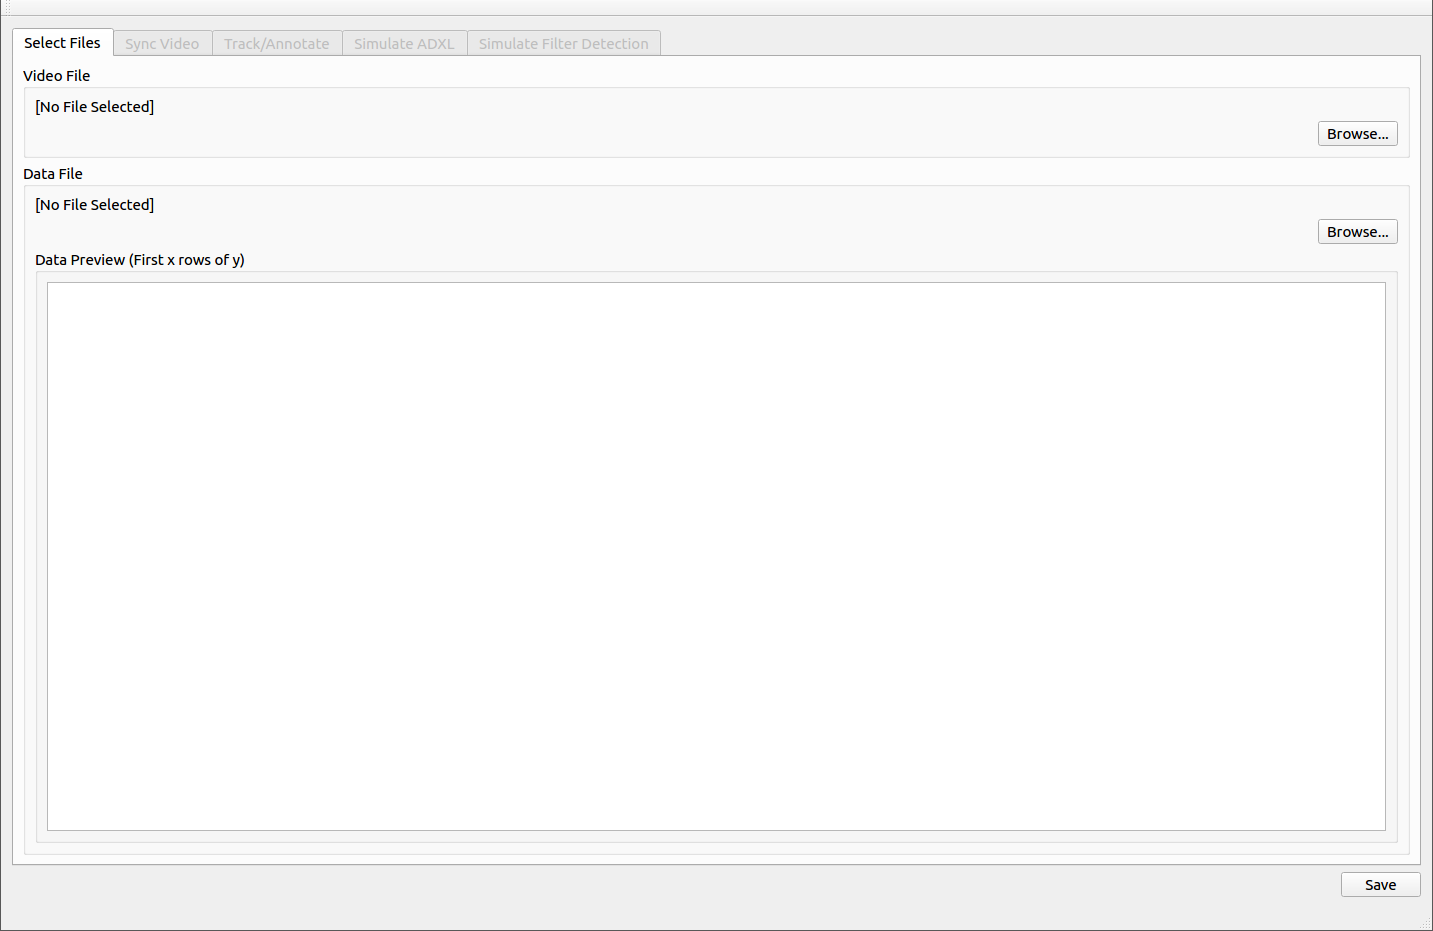
\includegraphics[width=1\linewidth]{importdata}
		\caption{The data management panel. Both video and data files must be present to proceed to further steps. When a valid data file is loaded, the first ten lines will be displayed.}
		\label{fig:importdata}
	\end{figure}
	\begin{enumerate}
		\item Create a new QValiData configuration file by pressing CTRL-N (Command-N on macOS), or clicking File $\rightarrow$ New in the menu bar.
		\item Save this file in the working folder (ideally, alongside the data and video to import) by pressing CTRL-S (Command-S), clicking the ``Save" button near the bottom of the window, or clicking File $\rightarrow$ Save in the menu bar. Ensure that the file is saved with the ``.conf" extension to make locating it easier.
		\item Import video by clicking the ``Browse..." button under the ``Video File" section \textbf{(Fig. \ref{fig:importdata})}. Select the video file in the file browser that appears.
		\item Import data by clicking the ``Browse..." button under the ``Data File" section \textbf{(Fig. \ref{fig:importdata})}. Select the data file in the file browser that appears. When a recognized data file format is imported, an excerpt of the data will be displayed in the window. 
		\item When video and logger data are successfully imported, the remaining tabs will become accessible.
	\end{enumerate}
	
	\subsection{Synchronization}
	\begin{figure}[H]
		\centering
		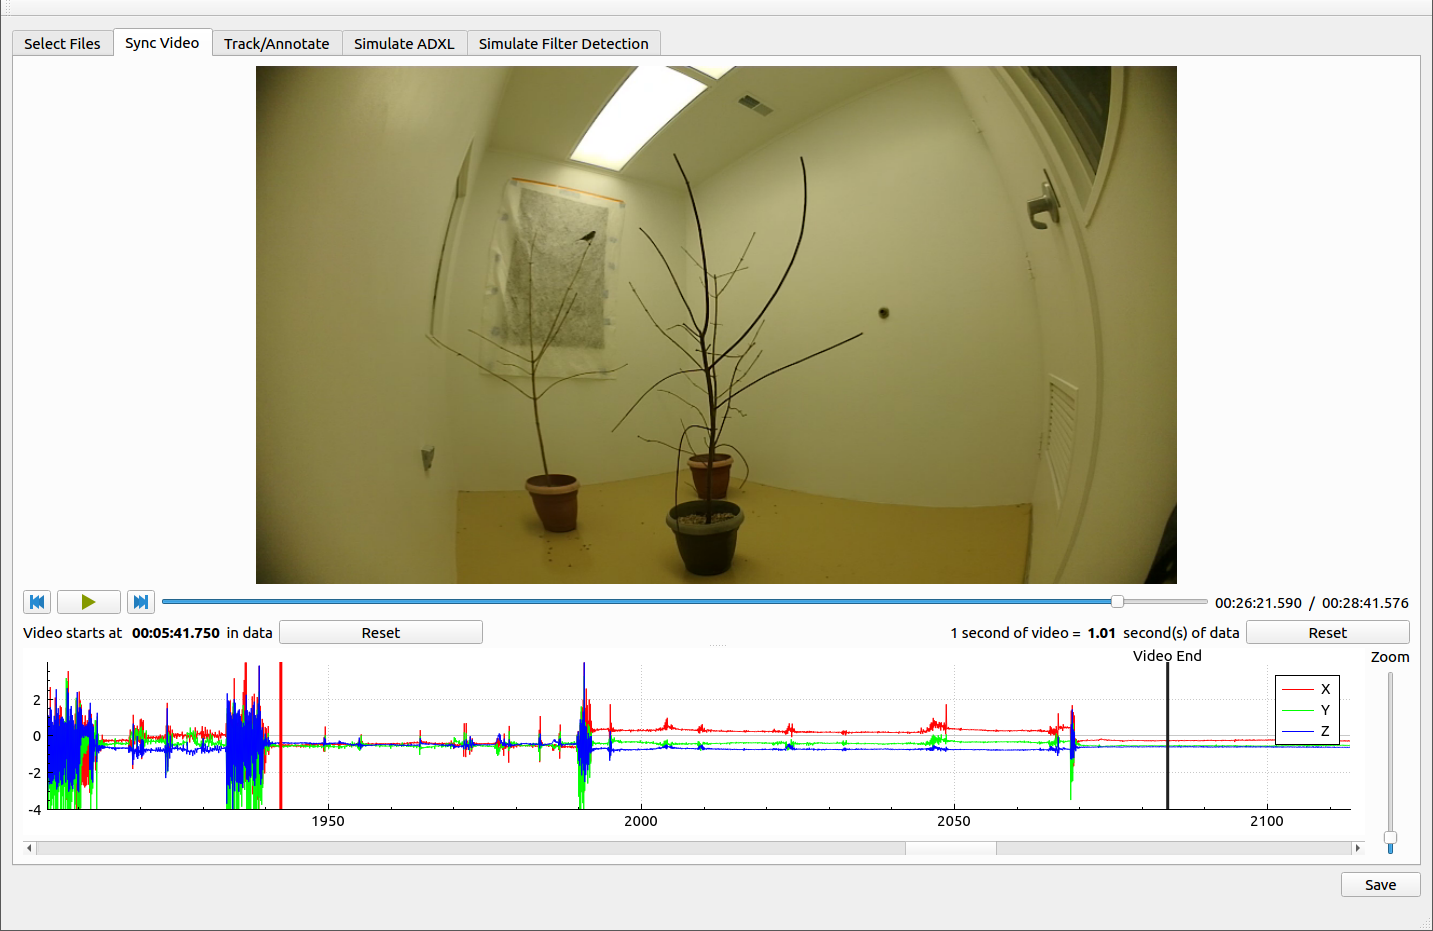
\includegraphics[width=1\linewidth]{syncvideo}
		\caption{The video synchronization task. Video (top) and data (bottom) are displayed together and can be time-aligned to ensure that activity visible on video corresponds to its associated data.}
		\label{fig:syncvideo}
	\end{figure}
	\begin{enumerate}
		\item Navigate to the ``Sync Video" tab at the top of the window. 
		\item Search for a recognizable event in the video, and look for its counterpart in the data. We will call this the ``Synchronizing Event``. 
			\begin{itemize}
				\item \textbf{TIP}: It is often much easier to create such events during the experimental phase through artificial means (eg. turning or shaking the logger in front of the camera), as such events are less likely to be encountered in the experiment itself.
			\end{itemize}
		\item Note the position of the vertical red line in the data plotter \textbf{(Fig. \ref{fig:syncvideo})}. Click the line to highlight it, and drag it towards the point in the data where the synchronizing event occurs. Click anywhere else on the graph to de-select the line.
		\item If the video plays too quickly/slowly compared to the data, adjust the data rate in a similar manner by adjusting the ``Video End" marker in the data plotter, denoted by a dark gray vertical line \textbf{(Fig. \ref{fig:syncvideo})}.
		\item It may be necessary to repeat the process several times in order to refine the synchronization.
	\end{enumerate}
	
	\subsection{Annotation}
	\begin{figure}[H]
		\centering
		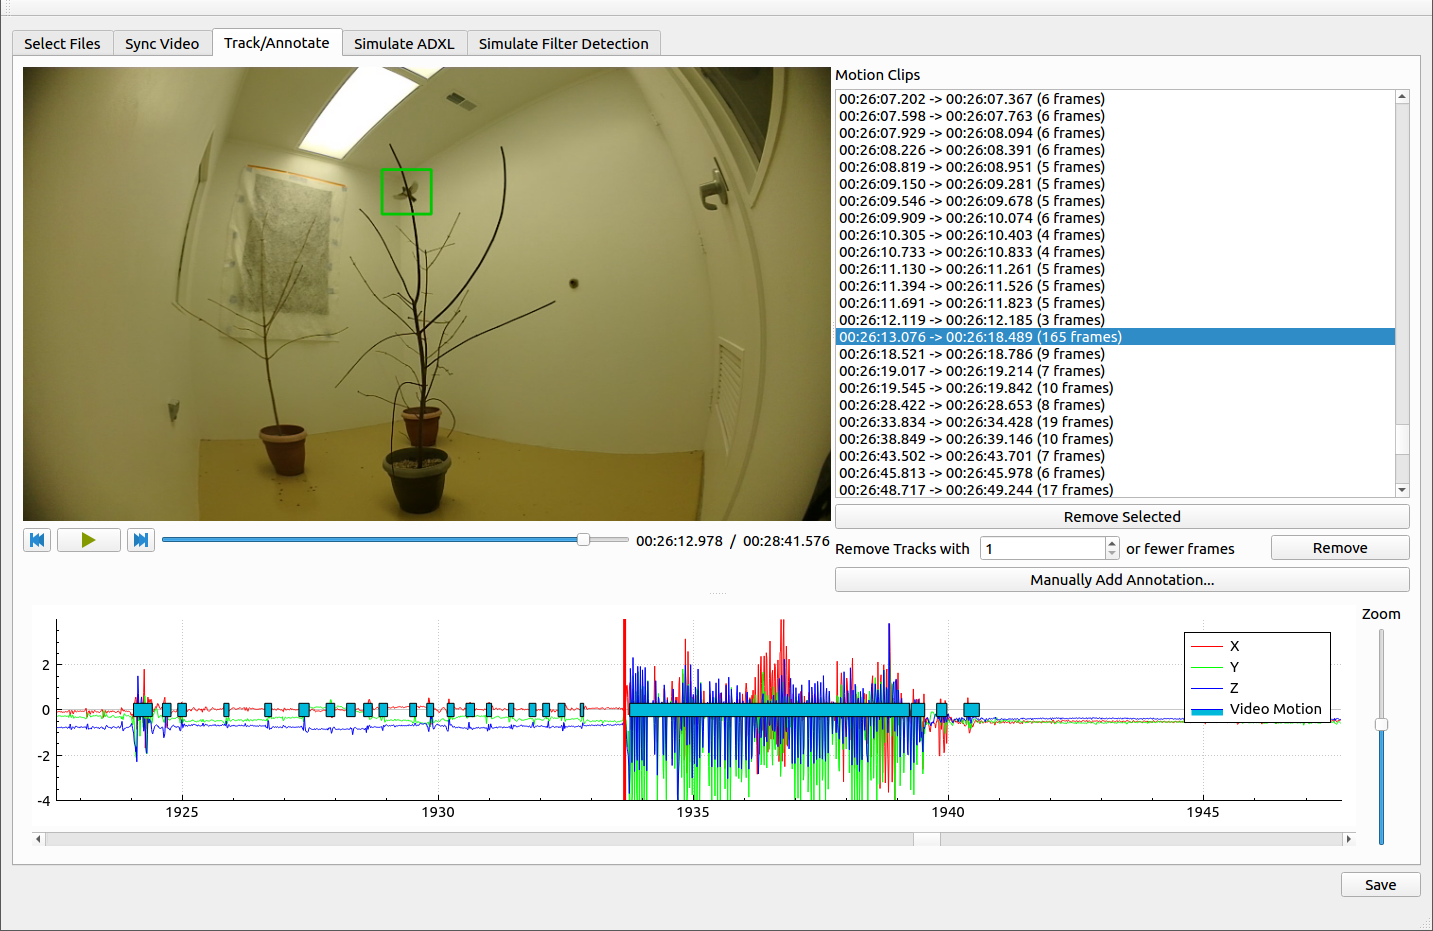
\includegraphics[width=1\linewidth]{selectbird}
		\caption{Annotation task. When performing Automatic Annotation, click the green squares to select areas of motion to track. Otherwise, annotations can be added manually by double-clicking on regions of data in the plotter.}
		\label{fig:annotate}
	\end{figure}
	
	\begin{figure}[H]
		\centering
		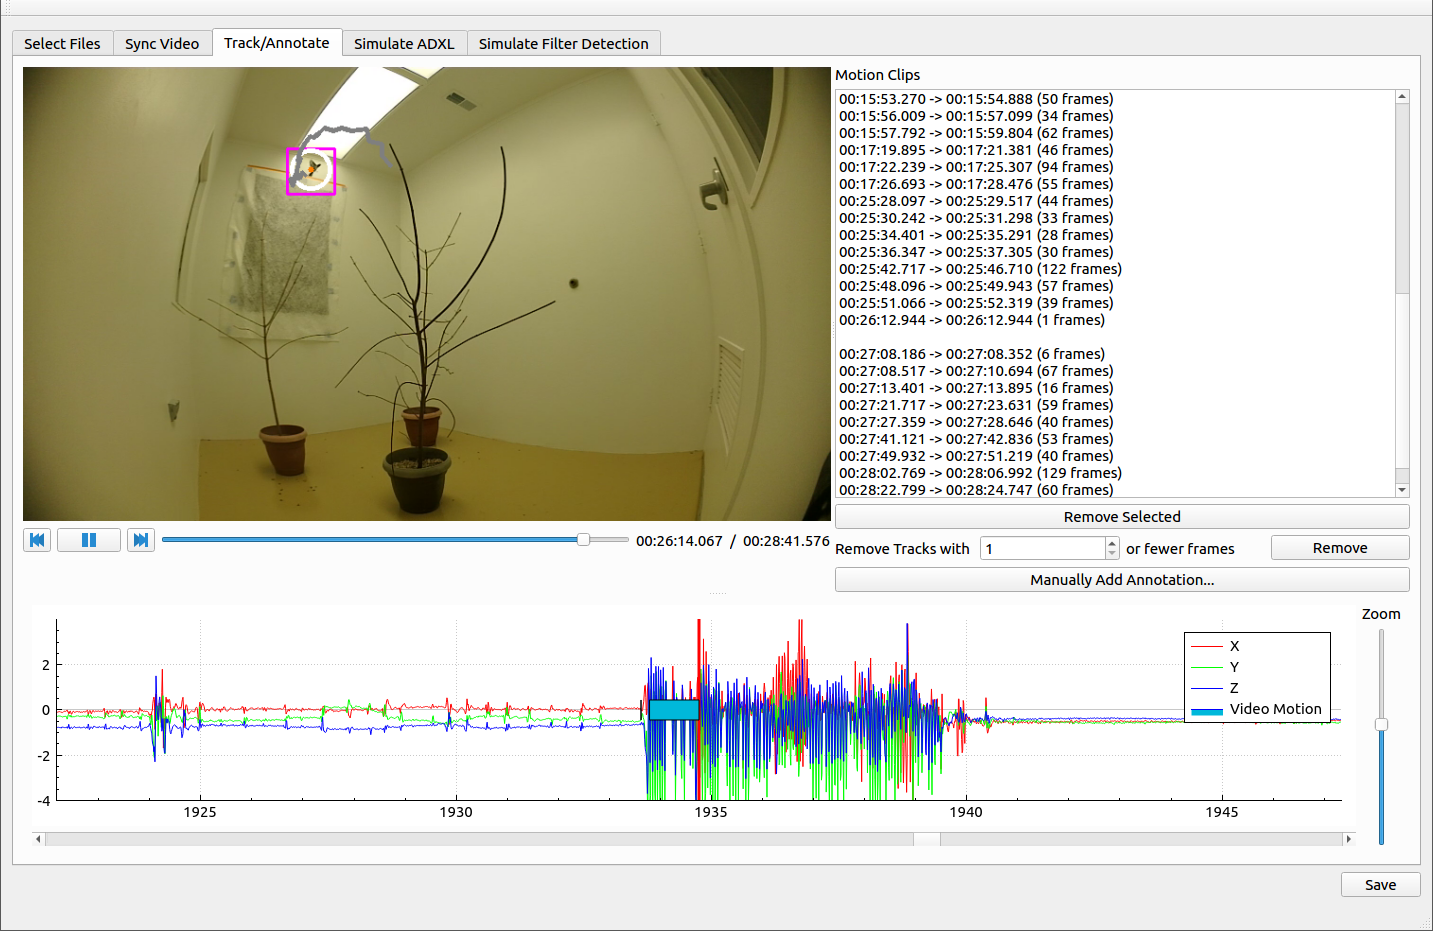
\includegraphics[width=1\linewidth]{tracking}
		\caption{Tracking the bird. When performing Automatic Annotation, the motion tracker will automatically generate annotations in the data plotter (small rectangles on data plotter) as well as record the position of the subject in each video frame.}
		\label{fig:tracking}
	\end{figure}
	
	\subsubsection{Automatic Annotation}
		QValiData has a built-in video tracker that can automatically locate movement and track objects in the video. This serves the dual purpose of marking periods of motion in data and magnifying video around the area of movement in subsequent steps, to enhance visibility of the subject.
		\begin{enumerate}
			\item Navigate to the ``Track/Annotate" tab at the top of the window.
			\item Press ``Play" to start looking for motion. If it is known that no activity of interest occurs in a particular section, it may be skipped by dragging the trackbar (below the video player), or clicking at a particular time in the data plotter. 
			\item If motion is detected, video playback will be paused, and areas of video with possible motion will be surrounded with boxes.
			\item Click the box that most closely encloses an area of motion \textbf{(Fig. \ref{fig:annotate})}. The tracker will automatically start the video and begin tracking the subject, drawing a white circle around the approximate center of movement. If the video does not start playing automatically, start playback by pressing the ``Play" button again.
			\item If the tracker encounters an error or loses track of the subject, video playback will automatically pause. The tracker may be ``re-trained" on another section of video with motion, or tracking may be stopped by skipping forward. Additionally, previous sections may be re-tracked by skipping backward in the video.
			\item While the tracker is actively tracking the subject \textbf{(Fig. \ref{fig:tracking})}, a bar will be placed on the data to indicate time periods in which tracking data is available.
		\end{enumerate}
	\subsubsection{Manual Annotation}
		Under some circumstances, the video tracker may not be able to reliably track the subject, or motion tracking may not be desired. QValiData provides an intuitive interface for manually adding annotations.
		\begin{enumerate}
			\item Navigate to the ``Track/Annotate" tab at the top of the window.
			\item Press the ``Manually Add Annotation..." button to enter Manual Annotation mode \textbf{(Fig. \ref{fig:annotate})}.
			\item Move the video/data trackbar so that the event of interest is visible. 
			\item On the data plotter, double-click at the time when the event starts.
			\item Move to the end of the event and double-click at that point in time. An annotation should appear over the event.
			\item After all annotations have been added, click the button again to exit Manual Annotation mode.
		\end{enumerate}
	\textbf{NOTE}: Remember to save annotations periodically, as unsaved changes will be lost if the program is closed.
	\subsection{Simulation}
		\begin{figure}[H]
			\centering
			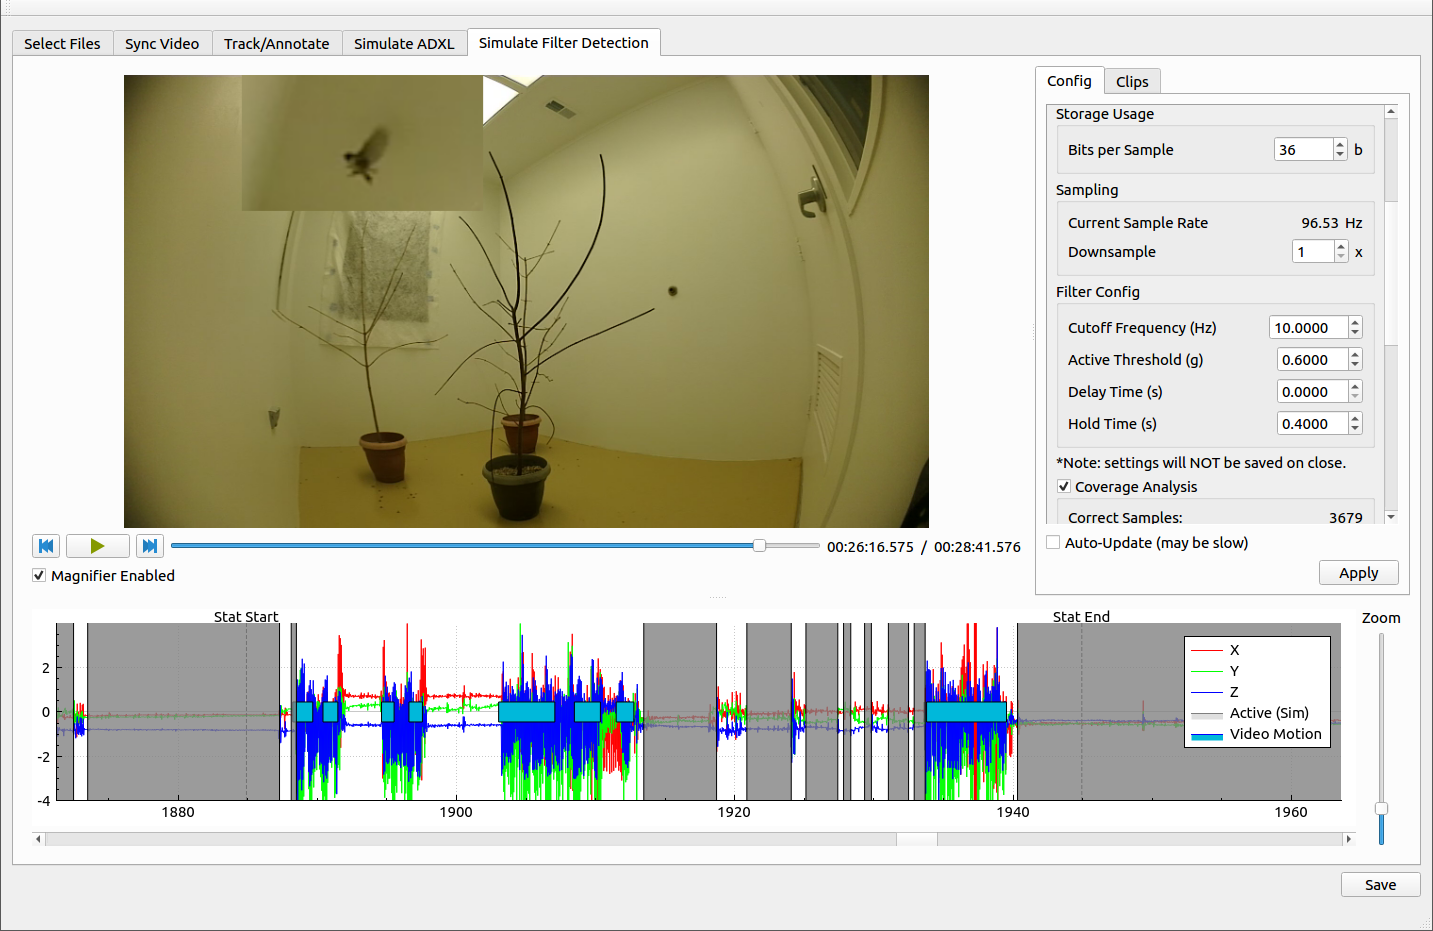
\includegraphics[width=1\linewidth]{simulate}
			\caption{Activity Detector simulation. The video viewer can be automatically magnified around the subject to improve visibility. The data plotter shows the results of a simulation run, with darker areas representing sections of data that were not detected by the activity detector. The dashed lines around ``Stat Start" and ``Stat End" indicate simulation boundaries. Only statistics about data between these portions is counted. These markers can be moved by double-clicking the left or right mouse button in the data plotter.}
			\label{fig:simulate}
		\end{figure}
		QValiData provides two logger simulations by default, although more can be added by modifying the source code. The first simulates the Awake Bit in the ADXL362 three-axis MEMS accelerometer, while the second simulates the behavior of a generic three-axis accelerometer with a high-pass filter to detect motion. 
		
		\begin{enumerate}
			\item Navigate to one of the simulation tabs at the top of the window.
			\item In the data plotter, move to the beginning of the experiment period and double-click at the desired point using the \textbf{LEFT} mouse button, to set the starting point of the simulation.
			\item Move to the end of the experiment period and double-click using the \textbf{RIGHT} mouse button to set the end of the simulation. 
			\item Adjust activity detection parameters, located in the right-hand side panel \textbf{(Fig. \ref{fig:simulate})}.
			\item Press ``Apply" to run the simulation. 
				\begin{itemize}
					\item The data plotter will darken in areas where the activity logger does not detect activity \textbf{(Fig. \ref{fig:simulate})}.
					\item If ``Coverage Analysis" is checked in the right-hand side panel, the simulation generates statistics on correctly- and incorrectly-identified events, using the video annotations as ground-truth. These values can be exported as the following files:
					\begin{itemize}
						\item \textbf{Coverage Data}: List all motion events detected by \textbf{manual or automatic annotation}, along with a percentage value indicating how much of each event was correctly identified by the \textbf{logger simulation}. This indicates how much of the events detectable in video are ``covered" by the simulated logger.
						\item \textbf{Active Region Data}: List all motion events reported by the \textbf{logger simulation}, along with a percentage value indicating how much of each event corresponds to \textbf{manual or automatic annotations} of events detected in video. This indicates how much the events detected by the logger simulator correspond to ground-truth video data.
					\end{itemize} 
				\end{itemize}
			\item Play through the video to validate activity detection. A ``magnifying glass" effect can be enabled to zoom areas of video surrounding the subject, which may assist in locating the subject in activity periods. 
				\begin{itemize}
					\item \textbf{NOTE}: Magnification is only available if automatic annotations are used. 
				\end{itemize}
		\end{enumerate}
		
\section{Development}
	\subsection{Compiling from Source}
		\subsubsection{Dependencies}
		\begin{enumerate}
			\item \textbf{Qt 5}: User interface library
				\begin{itemize}
					\item This can be downloaded from: \href{https://www.qt.io/download-qt-installer}{https://www.qt.io/download-qt-installer}
						\begin{itemize}
							\item \textbf{NOTE:} A Qt account is required, which may be created free of charge on the Qt website. The free Open Source licensing option is sufficient for QValiData.
						\end{itemize}
					\item Qt Creator is recommended for editing and building source code.
				\end{itemize}
			\item \textbf{OpenCV}: Computer Vision toolkit
				\begin{itemize}
					\item This can be downloaded from: \href{https://github.com/opencv/opencv}{https://github.com/opencv/opencv}
					\item \textbf{NOTE}: Some additional modules are required in addition to the ``core" OpenCV package, so it may be necessary to compile OpenCV from source:
						\begin{itemize}
							\item \texttt{imgcodecs}
							\item \texttt{imgproc}
							\item \texttt{plot}
							\item \texttt{tracking}
							\item \texttt{video}
							\item \texttt{videoio}
						\end{itemize}
					\item Detailed build instructions can be found at\\ \href{https://docs.opencv.org/master/d7/d9f/tutorial_linux_install.html}{https://docs.opencv.org/master/d7/d9f/tutorial\_linux\_install.html}\\
					(applicable to both Linux and macOS)
						\begin{itemize}
							\item It may also be necessary to install CMake, depending on platform. It is recommended to use the CMake GUI to configure build options. CMake (and CMake GUI) can be downloaded at: \href{https://cmake.org/download/}{https://cmake.org/download/}
						\end{itemize}
				\end{itemize}
			\item \textbf{iir1-dev}: Contains digital filters for simulations
				\begin{itemize}
					\item This can be downloaded from: \href{https://github.com/berndporr/iir1}{https://github.com/berndporr/iir1}
					\item Alternatively, it can be installed on Ubuntu or Debian by running:
					\begin{verbatim}
					sudo add-apt-repository ppa:berndporr/dsp
					sudo apt-get update
					sudo apt-get install iir1-dev
					\end{verbatim}
				\end{itemize}
		\end{enumerate}
		
		Once the dependencies have been installed, QValiData can be compiled from within the \texttt{QValiData} directory, either using \texttt{qmake} and \texttt{make}, or by importing the project file \texttt{qvalidata.pro} into Qt Creator
		
	\subsection{Adding More Simulation Models}
	A simulation model consists of a \textbf{User Interface} and a \textbf{Simulator Back-end}:
	\begin{itemize}
		\item \textbf{User Interface}: The display that is used to control the simulation and show its results. It consists of a Qt widget that inherits from the \texttt{SimulatorTab} class. Although this class is large and complex, nearly all simulator-specific code is contained in the function \texttt{on\_buttonApply\_clicked()}, which runs the simulation by calling the back-end when the ``Apply" button is clicked. The User Interface must provide appropriate configuration values to the simulator back-end before the simulation begins. The exact formatting of the configuration is explained in detail in the next sections.
		
		\item \textbf{Simulator Back-end}: The program that contains activity detector code to be simulated. It inherits from the \texttt{ActivityDetector} class, which has a simple interface that closely emulates the streaming-style data format received by a real sensor. 
	\end{itemize}
	\subsection{User Interface}
		The User Interface allows synchronized playback of video and logger data, and exposes some of the simulator back-end's configuration options to the user. An example user interface can be found at \texttt{QValiData/ActDetSimView/actdetsimview.cpp}, which configures the simulation of an accelerometer logger filtered by a digital high-pass filter. All simulator user interfaces must inherit from the \texttt{SimulatorTab} interface in order to operate properly.\\
		To add a new User Interface panel for custom simulations:
		\begin{enumerate}
			\item Duplicate the \texttt{ActDetSimView} folder and its contents.
			\item Re-name the source files and class to avoid conflicts (Re-name all occurrences of \texttt{ActDetSimView})
			\item Add the folder and files to the \texttt{QValiData.pro} file under the appropriate sections (Header, source, form, include directory)
			\item Modify the form to add/remove UI elements appropriate to the particular simulator back-end. 
			\item In the \texttt{.cpp} source file, under \texttt{on\_buttonApply\_clicked()}, edit the sections marked in comments to suit the particular simulator back-end being used. The most necessary changes are usually modifying the configuration routine to add or remove fields to be passed to the back-end as a configuration object. The structure of the configuration object to be passed is described in detail in the next section.
		\end{enumerate}
		
	\subsection{Back-End}
		The simulation back-end is designed to be similar in structure to the data collection programs that would normally run on real activity loggers. In particular, it only allows access to streaming data (ie one sample at a time) as is the case with real sensors, and it is able to preserve some state information between samples. A sample back-end is provided at \texttt{QValiData/ActDetSimView/accelfilterdetector.cpp}. The back-end uses the \texttt{ActivityDetector} class, which is inherited to create custom simulator back-ends. The following functions must be overridden from the interface:
		\begin{itemize}
			\item \texttt{bool config(QMap<QString, qreal> config)}\\
			Configures the activity detector using \texttt{config}, a map of string keys to real number values containing desired activity detector values and their labels. Keys may be any custom string that can uniquely identify a particular setting, so long as the User Interface provides the same label when the configuration map is created. For instance, if the activity detector has an adjustable threshold, a key-value pair with the configured threshold setting may be added to this object to set up the activity detector. Returns True if successful. Returning False will halt the simulation and show an error message to the user, with the opportunity to add custom text. For instance, a validity check may be added in this function to ensure configuration values are compatible. 
			
			\item \texttt{bool next(QMap<QString, qreal> sample)}\\
			Runs one ``step" of the simulation ie gives the activity detector one more sample. The argument \texttt{sample} is a mapping of string keys to real number values containing all sensor readings for a particular sample, as well as the time. Keys are named exactly as they appear in the data CSV file for each column of a particular sample. Returns True if successful, False if an error occurs. Returning False will halt the simulation and show an error message to the user, with the opportunity to add custom text.
			
			\item \texttt{bool isActive()}\\
			Returns True of the activity detector has detected significant activity at the moment this function is called.
			
			\item \texttt{QString getErrorString()}\\
			Returns the most recent error message, which will be displayed to the user in the event of an error. 
		\end{itemize}
		To add a new simulation back-end:
		\begin{enumerate}
			\item Create a new C++ class and save to a new folder within the \texttt{QValiData} directory. 
			\item Add the folder and files to the \texttt{QValiData.pro} file under the appropriate sections (Header, source, include directory)
			\item Include the \texttt{activitydetector.h} header. 
			\item Override and implement all virtual functions from the \texttt{activitydetector.h} header.
			\item To include custom error messages, declare a \texttt{QString} and set its value to the desired message when an error has been encountered. Then, return this \texttt{QString} object in \texttt{getErrorString()} is called.
		\end{enumerate}
		
	\subsection{Directory Structure}
	The QValiData project, as seen from the Git repository, is as follows:
		\begin{itemize}
			\item \texttt{QValiData/}: Contains the main Qt project and code associated with each tab in corresponding folders
				\begin{itemize}
					\item \texttt{ActDetSimView/}: Filtered activity detector simulator. This directory can also serve as a template for creating new simulation models.
					\item \texttt{ADXLSimView/}: ADXL362 activity detector simulator
					\item \texttt{FileSelector/}: File Selection tab
					\item \texttt{SyncView/}: Synchronization tab
					\item \texttt{TrackView/}: Video Annotation tab
				\end{itemize}
			\item \texttt{lib/}: Contains files that are depended on by multiple tabs or components
				\begin{itemize}
					\item \texttt{ActivityDetector}: Contains the \texttt{ActivityDetector} interface class, useful for creating new simulation models
					\item \texttt{ADXLSim}: ADXL362 simulator model
					\item \texttt{CloseupVideoViewer}: Video player with picture-in-picture magnifying around a point of interest
					\item \texttt{MotionPath}: Container for annotation points that stores coordinates of a subject's motion over a contiguous span of time
					\item \texttt{OpenCVDisplay}: Utility for displaying OpenCV Mat objects in a Qt widget with size-aware scaling
					\item \texttt{OpenCVVideoPlayer}: Utility for playing OpenCV videos in a Qt widget with size-aware scaling
					\item \texttt{QCPPlotTimeSeries}: Convenience class for displaying data in data plotter
					\item \texttt{QCustomPlot}: Plotting utility (\href{https://www.qcustomplot.com/}{https://www.qcustomplot.com/})
					\item \texttt{SimulatorTab}: Interface for creating new simulator user interfaces
					\item \texttt{TimeSeries}: Container for time-aligned data samples. Also includes a CSV import function.
					\item \texttt{VideoTracker}: Contains the motion tracking engine that identifies and annotates motion in video.
				\end{itemize}
			\item \texttt{doc/}: Contains documentation and resources for generating this PDF.
		\end{itemize}
		\newpage
	\section{Credits}
	QValiData uses:
		\begin{itemize}
			\item Qt 5 (Licensed under LGPLv3)
			\item qcustomplot (Licensed under GPLv3)
			\item OpenCV (Licensed under BSD 3-Clause)
			\item Iir1 (Licensed under the MIT License)
			\item linuxdeployqt (Licensed under GPLv3)
		\end{itemize}
	Special Thanks:
		\begin{itemize}
			\item Geoffrey Brown
			\item Adam Fudickar
			\item David Crandall
		\end{itemize}
\end{document}
